\documentclass[10pt]{article}
\usepackage{a4}
\usepackage{epsfig}
\usepackage{listings}
\usepackage{tabularx}
\lstset{language=Delphi}%
\lstset{basicstyle=\sffamily\small}%
\lstset{commentstyle=\itshape}%
\lstset{keywordstyle=\bfseries}%
%\lstset{blankstring=true}%
\newif\ifpdf
\ifx\pdfoutput\undefined
  \pdffalse
\else
  \pdfoutput=1
  \pdftrue
\fi
\begin{document}
\title{Programming GTK in Free Pascal:\\ Menus 
%and Marshallers
}
\author{Florian Kl\"ampfl\\and\\Micha\"el Van Canneyt}
\date{September 2000}
\maketitle
\section{Introduction}
In the third article on programming the GTK toolkit, the us of menus in GTK
is explored.
%two topics are
%explored: The programming of menus and the use of marshallers. 

Menus can be built in essentially 2 ways; the easier way through the
use of a itemfactory, and the more complex way, doing all necessary calls
manually. The advantages of both ways are discussed.

%Marshallers can be used to replace the default signal handling mechanisms 
%of GTK. The use of marshallers will be demonstrated by building a small
%object which will have custom handlers for certain events.

\section{Menus the easy way: The item factory}
The easy way to construct a menu is to use an item factory. An Item factory
gets as input an array of records, which describe a menu structure, and
returns a completely built menu, ready to be added to a window.

The great advantage of an item factory is that it is easy to use; a
disadvantage is that 
\begin{enumerate}
\item There is less control over the produced menu items; e.g. 
displaying a menu item with a small icon is not possible.
\item The callbacks of the constructed menu is different from the usual 
signal model, making it difficult to combine a menu entry with a
speedbutton. There are also 2 types of callback, so type checking is not
possible.
\item In Pascal, constant records must be specified using the names of the
members; this makes the array with the menu items to be rendered quite
complicated.
\end{enumerate}

To create a menu, first the item factory must be created. The function to do 
this is defined as follows:
\begin{lstlisting}{}
gtk_item_factory_new(container_type:TGtkType; 
                     path:Pgchar;
                     accel_group:PGtkAccelGroup):PGtkItemFactory;
\end{lstlisting}
The three arguments to this function have the following meaning:
\begin{description}
\item[container\_type] This identifies the kind of menu that will be
rendered. It can have one of the following values:
\begin{description}
\item[GTK\_MENU\_BAR\_TYPE] A menu bar will be created to hold all items.
\item[GTK\_MENU\_TYPE] A menu that can be used as a popup menu, or that can be
attached as a sub-menu to another menu, will be created.
\item[GTK\_OPTION\_MENU\_TYPE] Makes everything in a drop-down style menu which
can be used to select one value.
\end{description}
\item[path] is the name of the menu to be generated.
\item[accel\_group] Is a pointer to a group of accelerators. All
accellerators for the generated menu will be attached to this group.
\end{description}

The accelerator group needed for the item factory can be constructed 
using a simple call to \lstinline|gtk_accel_group_new|; this function 
takes no arguments,  and returns a pointer to a new accelerator group.

To actually create the menu, a call to
\lstinline|gtk_item_factory_create_items| is needed; This procedure is 
defined as follows:
\begin{lstlisting}{}
gtk_item_factory_create_items(ifactory:PGtkItemFactory; 
                              n_entries:guint; 
                              entries:PGtkItemFactoryEntry; 
                              callback_data:gpointer);
\end{lstlisting}
The first argument to this call, \lstinline|ifactory|, is the itemfactory; 
the second argument, \lstinline|n_entries|, is the number of items in the 
array of records describing the menu. The third argument, \lstinline|entries|,
is the actual array describing the menu. The last argument
\lstinline|callback_data| is a pointer that will be passed to the menu
callbacks.

The menu structure that should be created by the item factory is an 
array of records of the type  \lstinline|TGtkItemFactoryEntry|. 
This record is defined as follows:
\begin{lstlisting}{}
 TGtkItemFactoryEntry = record
    path : Pgchar;
    accelerator : Pgchar;
    callback : TGtkItemFactoryCallback;
    callback_action : guint;
    item_type : Pgchar;
 end;
\end{lstlisting}
The fields have the following meaning:
\begin{description}
\item[path]
The first entry is the path of the menu item. This indicates the place of
the menu entry in the whole menu. For instance, the menu item \textbf{New}
in the menu \textbf{File} would be designated by \lstinline|'/File/New'|.
So, the slash is used to separate the menu levels. 

To make one of the letters of the menu item name active, so the item can be
selected by pressing the letter (on the keyboard) when the menu is opened, 
the key to be used should be preceded by an underscore. 
In e.g. \lstinline|'/File/_New'|, the letter \textbf{N} could be used to 
select the  \textbf{New} item if the \textbf{File} menu is active.

\item[accelerator] To make a shortcut to the menu item so it can be 
activated at all times, the shortcut name can be specified in the 
\lstinline|accelerator| field. This can be any key, together with some 
modifiers. e.g. \lstinline|'<control>N'| will make the key combination 
'CTRL-N' a shortcut.

The accelerator should be speciefied as normal text.  A list of possible
modifiers can be found in table \ref{tab:modifiers}.
\begin{table}[ht]
\begin{center}
\caption{List of modifier strings for shortcut keys}\label{tab:modifiers}
\begin{tabular}{cc}
Modifier & alias \\ \hline
\lstinline|<control>| & \lstinline|<ctl>|, \lstinline|<ctrl>| \\
\lstinline|<shift>| & \lstinline|<shft>| \\
\lstinline|<alt>| & \lstinline|<mod1>| \\ \hline
\end{tabular}
\end{center}
\end{table}

\item[callback] Contains a pointer to the function that should be called
when the menu item is activated. The type of the menu handler is not the 
same as a normal signal handler; The actual callback should be of the type
\lstinline|TGtkItemFactoryCallback1|:
\begin{lstlisting}{}
procedure (callback_data:gpointer; 
           callback_action:guint; 
           widget:PGtkWidget);cdecl;
\end{lstlisting}
Which is not the same as the type of the \lstinline|callback| field, so
a typecast will always be necessary.

\item[callback\_action] This is passed on to the callback in the
\lstinline|callback_action| parameter.

\item[item\_type] is the type of menu item. Several types can be used; the
complete list can be found in \ref{tab:menutypes}, but the must important
ones are \lstinline|'<Item>'|, which specifies a normal menu item, 
 and \lstinline|'<Branch>'|, which indicates a sub-menu.
\begin{table}[ht]
\begin{center}
\caption{Possible menu item types}\label{tab:menutypes}
\begin{tabularx}{\textwidth}{lX}%
Item type & Menu kind \\ \hline
\lstinline|'<Item>'| & indicates a normal item. An empty string or \lstinline|Nil|
have the same meaning. \\
\lstinline|'<CheckItem>'| & a check menu item. \\
\lstinline|'<ToggleItem>'| & a toggle menu item (same as check menu). \\
\lstinline|'<RadioItem>'| & a radio item. \\
\lstinline|'<Separator>'| & a separator bar. \\
\lstinline|'<Branch>'| & an item to hold a submenu.\\
\lstinline|'<LastBranch>'| & an item to hold a submenu, but right aligned.\\ \hline
\end{tabularx}
\end{center}
\end{table}
\end{description}
Now all elements to create a menu are introduced, and the menu can be
created. The following definitions should now be clear:
\begin{lstlisting}{}
Var
Window  : PGtkWidget;
MenuBar : PGtkWidget;

Type
  FC = TGtkItemFactoryCallback;

Const
 NrMenuItems = 21;
  TheMenu : Array[1..NrMenuItems] of TGtkItemFactoryEntry = (
    (path:'/_File';Accelerator:Nil;
     Callback:Nil;Callback_action:1;item_type:'<Branch>'),
    (path:'/File/_New';Accelerator:'<ctrl>N';
     Callback:FC(@Menu);Callback_action:1;item_type:Nil),
    { ... }
\end{lstlisting}
Here the \lstinline|FC| type is introduced to make the typecast of the
\lstinline|Menu| handler easier; the 
\lstinline|TheMenu| constant is not given completely, since it is too long
and not instructive. The complete structure can be found in the sources
accompanying this article.

Using the above definitions, the menu can now be constructed:
\begin{lstlisting}{}
Procedure MakeMenu;

Var
  Factory : PGtkItemFactory;
  Accel   : PGtkAccelGroup;

begin
  Accel:=gtk_accel_group_new;
  Factory :=gtk_item_factory_new(GTK_MENU_BAR_TYPE,'<main>',accel);
  gtk_item_factory_create_items(Factory,NrMenuItems,@TheMenu,Nil);
  gtk_window_add_accel_group(GTK_Window(Window),accel);
  MenuBar:=gtk_item_factory_get_widget (Factory, '<main>');
end;
\end{lstlisting}
The \lstinline|gtk_window_add_accel_group| call attaches the accelerator
group that was filled up by the item factory to the window.

The \lstinline|gtk_item_factory_get_widget| call finally fetches the
object created by the item factory and stores it in a widget variable.

The \lstinline|Menu| callback used in the menus is defined as follows:
\begin{lstlisting}{}
procedure menu(Data : GPointer; 
               Action : Guint; 
               Widget : pGtkWidget); cdecl;
    
Var 
  TheLabel : PgtkWidget;
  LabelText : Pchar;
  S : AnsiString;
     
begin
  TheLabel:=g_list_nth_data(
             gtk_container_children(
               GTK_CONTAINER(Widget)),0);
  gtk_label_get(gtk_Label(theLabel),@LabelText);
  S := 'Chosen menu : ' + Strpas(Labeltext);
  gtk_label_set_text(GTK_LABEL(DisplayLabel),pchar(S));
end;
\end{lstlisting}
The \lstinline|DisplayLabel| is a label located on the window, it is used to
give some feedback on the used menu. The code to extract the menu name from
the menu widget passed to the handler will be explained later on. 

The result of all this is shown in figure \ref{fig:ex1}.
\begin{figure}
\caption{The menu made by the item factory.}\label{fig:ex1}
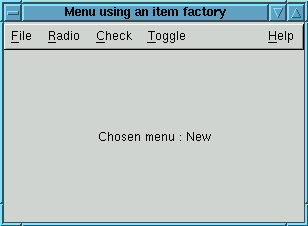
\epsfig{file=gtk3ex/ex1.png}
\end{figure}

As can be seen from the code above, the creation of a menu using an item
factory in GTK is not so hard. The drawback of the above method lies mainly
in the fact that Pascal handles constant records differently than C, which 
makes the array that describes the menu structure rather difficult to read.

The second drawback is that there is little control over the created items.

\section{Menus the hard way: manually}
When creating menus manually, mainly 4 objects are involved:
\begin{itemize}
\item The menu items themselves. To a menu item, a menu can be assiciated,
creating a sub-menu.
\item Menus, which contain a collection of menu items,
\item A accelerator group. This will be used to keep a collection of
shortcut keys for the menu items.
\item A menu bar, which can hold several menu items and their associated
menus. 
\end{itemize}
The last object is optional, if e.g. a pop-up menu is wanted.

To create a menu in a window, the following steps are involved:
\begin{enumerate}
\item Create an accellerator group. The accelerator group should be
connected to the window. \label{stepone}
\item Create a menu bar, and attach it to the window.
\item For each menu that should appear in a menu bar, do the following:
\begin{itemize}
\item Create a menu item, which will be shown in the menu bar.
\item Create a menu to hold the items that should pop up when the menu is
activated.
\end{itemize}
\item To each menu created in the previous step, add as many menu items as
needed. Add an accelarator to the group created in step \ref{stepone}.
\end{enumerate}

To make these steps easier (each of them involves quite some calls to GTK
functions) some functions will be introduced that make this easier.

The first function is the most simple one; it attaches a separator to a
menu:
\begin{lstlisting}{}
Function AddSeparatorToMenu(Menu:PgtkMenu):PgtkMenuItem;

begin
  Result:=pgtkmenuitem(gtk_menu_item_new); 
  gtk_menu_append(Menu,pgtkWidget(result));
  gtk_widget_show(PgtkWidget(result));
end;
\end{lstlisting}
The function takes one parameter, \lstinline|Menu|, the menu to which the
separator will be attached. A separator is created by simply creating an
empty menu item. Creating a new (empty) menu item is done with the
\lstinline|gtk_menu_item_new| call. 

With the \lstinline|gtk_menu_append| call, the newly created item is then 
added to the menu. Lastly, the item is shown; it will not become actually
visible till the menu is activated. If this is omitted, it will also not
be visible when the menu is activated.

Adding a menu with a shortcut key to a menu is a little more involved. Some
more elements are needed:
\begin{enumerate}
\item The menu to which to attach the menu item.
\item The accelarator group to which the accelerator key should be added.
\item The caption of the menu. An underscore character will indicate the 
letter of themenu that will be used as a shortcut to activate the item.
\item The shortcut for the menu item. An empty string means no shortcut.
\item A callback function which will be called when the menu item is
activated, and callback data which will sent to the callback.
\end{enumerate}
All these elements are found in the declaration of the following function:
\begin{lstlisting}{}
Function AddItemToMenu (Menu : PGtkMenu;
                        ShortCuts : PGtkAccelGroup;
                        Caption : AnsiString;
                        ShortCut : AnsiString;
                        CallBack : TgtkSignalFunc;
                        CallBackdata : Pointer
                       ) : PGtkMenuItem; 

Var
  Key,Modifiers : guint;
  LocalAccelGroup : PGtkAccelGroup;
  TheLabel : PGtkLabel;
  
begin
\end{lstlisting}
The variables declared in this function will be explained as the code is
presented.

First of all, a menu item must be created. Since a caption for the menu is
provided, the \lstinline|gtk_menu_item_new_with_label| will be used to
create a menu that has a label as a child:
\begin{lstlisting}{}
  Result:=pgtkmenuitem(gtk_menu_item_new_with_label(''));
  TheLabel:=GTK_LABEL(GTK_BIN(Result)^.child);
  Key:=gtk_label_parse_uline(TheLabel,Pchar(Caption));
\end{lstlisting}
After the menu item is created, the child label is fetched. The label caption is
then set using the \lstinline|gtk_label_parse_uline| function. This function 
will search a text for underscore characters, remove them from the text, and
then set the label's caption with the result. All letters which had an
underscore character prepended will be underlined in the label.

The function returns the first letter that had an underscore prepended. It
is stored, so it can be used to make an accelerator:
\begin{lstlisting}{}
If Key<>0 then
  begin
  LocalAccelGroup:=gtk_menu_ensure_uline_accel_group(Menu);
  gtk_widget_add_accelerator(PGtkWidget(result),'activate_item',
                             LocalAccelGroup,Key,
                             0,TGtkAccelFlags(0));
  end;
\end{lstlisting}
The call to \lstinline|gtk_menu_ensure_uline_accel_group| returns the 
accelarator group associated with the menu. If no group existed yet, one
will be created. The \lstinline|gtk_widget_add_accelerator| call takes the
following parameters:
\begin{itemize}
\item A pointer to a widget to which the accelerator should be attached.
\item The name of the signal which will be triggered when the shortcut 
is activated.
\item The accelerator group to which the shortcut should be installed,
usually this will be the accelerator group for the window to which the
widget is attached, but in this case this is the accelerator group of the
menu (which will only be active when the menu is actually shown)
\item The key from the shortcut.
\item The modifiers that should be pressed together with the key. For the
menu, this should be 0, since just the key should be hit.
\item The accelerator flags.
\end{itemize}

After the menu item was created and it's underlined key was made into an
accelerator, the menu can be attached to the menu:
\begin{lstlisting}{}
gtk_menu_append(Menu,pgtkWidget(result));
\end{lstlisting}

If a shortcut key was passed along to the procedure, can be added to the
window's accelerator group with the following code:
\begin{lstlisting}{}
If (ShortCut<>'') and (ShortCuts<>Nil) then  
  begin
  gtk_accelerator_parse (pchar(ShortCut), @key, @modifiers);
  gtk_widget_add_accelerator(PGtkWidget(result),'activate_item',
                             ShortCuts,Key,
                             modifiers, GTK_ACCEL_VISIBLE);
  end;
\end{lstlisting}
The call to \lstinline|gtk_accelerator_parse| will parse a string which
describes a shortcut key, and returns the corresponding key and modifiers,
which can then be passed on to the \lstinline|gtk_widget_add_accelerator|
call.

After the accellerator has been installed, the only thing that remains to be
done is to connect the callback to the activation of the menu:
\begin{lstlisting}{}
If CallBack<>Nil then
  gtk_signal_connect(PGtkObject(result),'activate',
                     CallBack,CallBackdata);
gtk_widget_show(PgtkWidget(result));  
end;
\end{lstlisting}
As the last line in the procedure, the newly created menu item is shown.
If the menu isn't visible yet, this will do nothing, but will ensure that
the item is also visible when the menu is visible.

Now a menu-item and a separator can be added to a menu. What remains to be
done is to add a menu to a menu bar. This is done in the following
procedure, which is given in its entirety:
\begin{lstlisting}{}
Function AddMenuToMenuBar(MenuBar : PGtkMenuBar;
                          ShortCuts : PGtkAccelGroup;
                          Caption : AnsiString;
                          CallBack : TgtkSignalFunc;
                          CallBackdata : Pointer;   
                          AlignRight : Boolean;     
                          Var MenuItem : PgtkMenuItem
                          ) : PGtkMenu; 

Var
  Key : guint;
  TheLabel : PGtkLabel;

begin
  MenuItem:=pgtkmenuitem(gtk_menu_item_new_with_label(''));
  If AlignRight Then
    gtk_menu_item_right_justify(MenuItem);
  TheLabel:=GTK_LABEL(GTK_BIN(MenuItem)^.child);
  Key:=gtk_label_parse_uline(TheLabel,Pchar(Caption));
  If Key<>0 then
    gtk_widget_add_accelerator(PGtkWidget(MenuItem),'activate_item',
                               Shortcuts,Key,
                               GDK_MOD1_MASK,GTK_ACCEL_LOCKED);
  Result:=PGtkMenu(gtk_menu_new);
  If CallBack<>Nil then
    gtk_signal_connect(PGtkObject(result),'activate',
                        CallBack,CallBackdata);
  gtk_widget_show(PgtkWidget(MenuItem));  
  gtk_menu_item_set_submenu(MenuItem, PgtkWidget(Result));
  gtk_menu_bar_append(MenuBar,PgtkWidget(MenuItem));
\end{lstlisting}
The code for this procedure quite similar as the previous one. The main
differences are:
\begin{itemize}
\item The result is not a menuitem, but a whole menu. The menuitem that is
displayed in the menu bar itself is returned in the \lstinline|MenuItem|
parameter.
\item The shortcut key for the underlined item is added to the window's
accelerator group, and has the \textsc{Alt} key (or \textsf{Mod1}) as 
the modifier key.
\item the created menu is attached to the menu item as a sub menu, and it is
the menu-item which is attached to the menu bar.
\end{itemize}

With the above calls, a menu can be constructed with a simple set of calls:
\begin{lstlisting}{}
FileMenu:=AddMenuToMenuBar(MenuBar,accel,'_File',Nil,
                           Nil,False,TempMenuItem);
AddItemToMenu(FileMenu,accel,'_New','<control>N',
              TgtkSignalFunc(@menu),DisplayLabel);
AddItemToMenu(FileMenu,accel,'_Open','<control>O',
              TgtkSignalFunc(@menu),DisplayLabel);
AddItemToMenu(FileMenu,accel,'_Save','<control>S',
              TgtkSignalFunc(@menu),DisplayLabel);
AddSeparatorToMenu(PGtkMenu(FileMenu));
AddItemToMenu(FileMenu,accel,'_Quit','<control>Q',
              TgtkSignalFunc(@destroy),Nil);
{ ... } 
\end{lstlisting}
The complete list of calls to create the menu can be found in the sources
accompagnying this article.

The second program is of course bigger than the first, due to all the code
to create the menus. Nevertheless, the manual way of creating has it's
advantages: it's quite easy to extend the AddItemToMenu to add a bitmap to
the menu entry as well. Using a itemfactory, there is (currently) no way to
add images to a menu.

Adding a bitmap to a menu is quite easy, and requires only a few extra
lines of code. The key point is that the gtkmenuitem object is just an empty
container (it descends from gtkbin), which does not display anything by itself. The
\lstinline|gtk_menu_item_new_with_label| call creates a menu item and puts a
gtklabel in it to display the menu item caption. Instead of a label object,
almost any other object can be put in the item. This fact is used in the
following code to add a bitmap in front of the menu caption, in a new
procedure to be called \lstinline|AddImageItemToMenu|:
\begin{lstlisting}{}
  Result:=pgtkmenuitem(gtk_menu_item_new);
  hbox:=PGtkHBox(gtk_hbox_new(false,0));  
  gtk_container_add(pgtkcontainer(result),pgtkWidget(hbox));
  pixmap:=gdk_pixmap_create_from_xpm(Nil,@BitmapData,Nil,pchar(BitMap));
  Image := PgtkPixMap(gtk_pixmap_new(Pixmap,BitmapData));
  gtk_box_pack_start(PGtkBox(hbox),pgtkWidget(image),false,false,0);
  TheLabel:=PgtkLabel(gtk_label_new(''));
  gtk_box_pack_start(PGtkBox(hbox),pgtkWidget(TheLabel),True,True,0);
  Key:=gtk_label_parse_uline(TheLabel,Pchar(Caption));
\end{lstlisting}
In the first line, a plain menu item is created with
\lstinline|gtk_menu_item_new|. In the following two lines,
a \lstinline|GTKHBox| is added to the menu item, and a reference to the box
is stored in the \lstinline|hbox| variable.

Then, a pixmap is created from a filename. The filename is passed in the 
\lstinline|BitMap| parameter to our routine. Using the newly created pixmap,
an Image is created, which can then be added to the box.

Finally, a regular GTK label is created to hold the caption of the menu
item, and added to the box. After that the procedure continues as for a
normal menu.

The complete code for the above \lstinline|AddImageItemToMenu| routine can
be found in the sources of the third example, accompagnying this article.
The result can be seen in figure \ref{fig:pixmenu}
\begin{figure}[ht]
\caption{The menu with bitmaps}\label{fig:pixmenu}
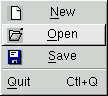
\epsfig{file=gtk3ex/ex3.png}
\end{figure}

Some notes regarding this algorithm are in order:
\begin{enumerate}
\item It would be possible to have not a filename passed to the routine, but
directly pass a pixmap object as well; for instance when using a toolbar,
toolbuttons corresponding to the menu entries could share the same pixmaps
as the menu entries.
\item Some alignment issues may arise when the menu contains items with and
without bitmaps. The above code does not address these issues. To solve
them, the regular menu items should also be constructed e.g. using a hbox or a
table with an empty cell. Also, an algorithm to determine whether any item of
the menu has an image would be needed.
\item The shortcut key is no longer shown in the menu widget; The reason for
this is unknown to the authors of this article; unfortunately the lack of
documentation on GTK prevents the implementation of a remedy.
\item The menu callback can no longer retrieve the menu text using a
straightforward approach, since the label displaying the caption is 
no longer the only child widget of the menu item. The callback has been
adapted for this in the example.
\end{enumerate}
Taking into account the above arguments should make it possible to write
better menu-creating routines which would replace the item factory
completely, and which would enable the use of bitmaps in menu items.

\end{document}
